% Created 2018-01-18 Thu 22:19
% \documentclass[aspectratio=169,10pt,trans]{beamer}
% \documentclass[aspectratio=169,10pt,trans]{beamer}
\documentclass[aspectratio=169,10pt]{beamer}

%% for handouts mode
% \documentclass[aspectratio=169,10pt,handout]{beamer}


% LiU theme packages
\usepackage{myLiU}%\usetheme{Madrid}
\usepackage[utf8]{inputenc}
\usepackage[T1]{fontenc}
%\usepackage{fixltx2e}
\usepackage{graphicx}
%\usepackage{longtable}
\usepackage{float}
%\usepackage{wrapfig}
%\usepackage{rotating}
\usepackage{fontawesome5}
% \usepackage[normalem]{ulem}
\usepackage{amsmath}
%\usepackage{textcomp}
% \usepackage{marvosym}
% \usepackage{wasysym}
\usepackage{amssymb}
\usepackage{hyperref}
\usepackage[round]{natbib}
\usepackage{color}
\usepackage{listings}
\lstset{language=Matlab,%
  % basicstyle=\color{red},
  breaklines=true,%
  morekeywords={matlab2tikz},
  keywordstyle=\color{blue},%
  morekeywords=[2]{1}, keywordstyle=[2]{\color{black}},
  identifierstyle=\color{black},%
  stringstyle=\color{mylilas},
  commentstyle=\color{mygreen},%
  showstringspaces=false,%without this there will be a symbol in the places where there is a space
  numbers=left,%
  numberstyle={\tiny \color{black}},% size of the numbers
  numbersep=5pt, % this defines how far the numbers are from the text
  emph=[1]{for,end,break},emphstyle=[1]\color{red}, %some words to emphasise
  % emph=[2]{word1,word2}, emphstyle=[2]{style},    
}

\tolerance=1000
% \usetheme{default}
\author[Arvind B]{Arvind Balachandran}
\date{April 28, 2023}
\title[BI-MMC Lab]{The BI-MMC Laboratory}
\subtitle{An experimental platform to implement and investigate the next generation algorithms for control and saftey of EVs.}
%\hypersetup{
%  pdfkeywords={},
%  pdfsubject={}}
 \AtBeginSection[]% "Beamer, do the following at the start of every section"
 {\begin{frame}% <beamer> 
     \frametitle{Outline} % make a frame titled "Outline"
     \tableofcontents[currentsection]  % show TOC and highlight current section
     \tableofcontents
   \end{frame}}

\usepackage{siunitx}

\usepackage{tikz}
\usetikzlibrary{calc,quotes,angles}

% definitions file
% \usepackage{xspace}
\newcommand{\uvec}[1]{\textit{$\textit{u}_{\textit{#1}}$}\xspace}
\newcommand{\tsim}{\textit{$\textit{t}$}\xspace}
\newcommand{\mass}{\textit{$\textit{m}$}\xspace}

%-------------------------------------------
% Handouts 
% \usepackage{handoutWithNotes}
% \usepackage{pgfpages}
% \pgfpagesuselayout{4 on 1}[a4paper,border shrink=5mm]

% temporarily disable overlays
% \newcommand*{\disableanim}[1]{{%
% 		\RenewDocumentCommand{\onslide}{ R<>{} }{}%
% 		#1%
% }}

%% Animation package 
\usepackage{animate}

% \AtBeginPart{\frame{\partpage}}

\setbeamertemplate{section page}{  
  \begingroup    
  \centering
  \begin{beamercolorbox}[sep=12pt,center,colsep=-4bp,rounded=true,shadow=flase]{section title}       
    \usebeamerfont{section title}\insertsection\par     
  \end{beamercolorbox}   
  \endgroup 
}
\AtBeginSection{\frame{\sectionpage}}

\begin{document}

\maketitle

% \include{frames/outline.tex} % outline
% \include{frames/motivation.tex} % 2-level inverter challenges
\begin{frame}{}
    \begin{alertblock}{PEP: Pendulum turn?}
        Experiment with vehicle parameters (especially inertia) to see if it occurs. (Are many rally drivers wrong?)
    \end{alertblock}
    \begin{columns}
        \begin{column}[c]{0.5\textwidth}
            Single Track Model:
            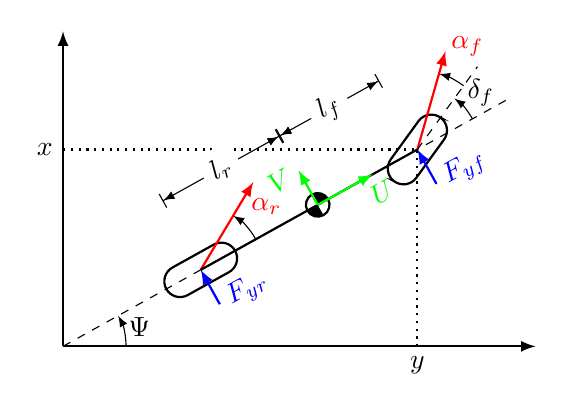
\begin{tikzpicture}

                \pgfmathsetmacro{\y}{4.5}
                \pgfmathsetmacro{\x}{2.5}
                \pgfmathsetmacro{\Angle}{atan2(\x,\y)}
                \pgfmathsetmacro{\AngleR}{30}
                \pgfmathsetmacro{\AngleF}{45}
                \pgfmathsetmacro{\AngleDelta}{25}
                \pgfmathsetmacro{\COMradius}{0.15}
                
                \coordinate (Origin) at (0,0);
                \draw [-latex,thick] (Origin)--++(0,\x+1.5) coordinate (yaxis); 
                \draw [-latex,thick] (Origin)--++(\y+1.5,0) coordinate (xaxis); 
                \draw [dashed] (Origin)--++(\Angle:6.5cm) coordinate (AngleEnd);
                \draw [dotted,thick] (\y,0) node [below] {$y$} --++(0,\x) coordinate (Fyf);
                \draw [dotted,thick] (0,\x) node [left] {$x$} --++(\y,0);
                \draw pic["$\Psi$", draw=black, text=black, -latex, angle eccentricity=1.25, angle radius=0.8cm]
                              {angle=xaxis--Origin--Fyf};
                
                % Fyr
                \coordinate (Fyr) at ($ (Origin) + (\Angle:2cm) $);
                \node at (Fyr) [rotate=\Angle,draw,thick,rounded corners=2mm,minimum width=1cm, minimum height=0.4cm] {};
                \draw [red,-latex,thick] (Fyr)--++(\Angle+\AngleR:1.3cm) coordinate (RedArrowOne);
                \draw pic["$\alpha_r$", draw=black, text=red, -latex, angle eccentricity=1.45, angle radius=0.8cm]
                              {angle=Fyf--Fyr--RedArrowOne};
                \draw [latex-,thick,blue] (Fyr)--++(\Angle-90:0.5cm) node [rotate=\Angle,right] {$F_{yr}$};           
                
                \draw [thick] (Fyr)--(Fyf); 
                
                % Fyf  
                \node at (Fyf) [rotate=\Angle+\AngleDelta,draw,thick,rounded corners=2mm,minimum width=1cm, minimum height=0.4cm] {};         
                \draw [red,-latex,thick] (Fyf)--++(\Angle+\AngleF:1.3cm) coordinate (RedArrowTwo);
                \draw [dashed] (Fyf)--++(\Angle+\AngleDelta:1.3cm) coordinate (DeltaAngleEnd);
                \draw pic["$\delta_f$", draw=black, text=black, -latex, angle eccentricity=1.35, angle radius=0.8cm]
                           {angle=AngleEnd--Fyf--DeltaAngleEnd};
                \draw pic["$\alpha_f$", draw=black, text=red, -latex, angle eccentricity=1.45, angle radius=1cm]
                      {angle=DeltaAngleEnd--Fyf--RedArrowTwo};
                \draw [latex-,thick,blue] (Fyf)--++(\Angle-90:0.5cm) node [rotate=\Angle,right] {$F_{yf}$};       
                
                % COM
                \coordinate (COM) at ($ (Origin) + (\Angle:3.7cm) $);
                \begin{scope}[rotate=\Angle]
                \fill [radius=\COMradius] (COM) -- ++(\COMradius,0) arc [start angle=0,end angle=90] -- ++(0,-2*\COMradius) arc [start angle=270, end angle=180];
                \draw [thick,radius=\COMradius] (COM) circle;
                \end{scope}
                \draw [-latex,thick,green] (COM)--++(\Angle+90:0.5cm) node [left,rotate=\Angle] {$V$};
                \draw [-latex,thick,green] (COM)--++(\Angle:0.8cm) node [below,rotate=\Angle] {$U$};
                
                % Labels
                \coordinate (LrLabel) at ($ (Fyr) +  (\Angle+90:1cm) $);
                \coordinate (COMLabel) at ($ (COM) +  (\Angle+90:1cm) $);
                \coordinate (LfLabel) at ($ (Fyf) +  (\Angle+90:1cm) $);
                \draw [{Bar}{latex}-{latex}{Bar}] (LrLabel)--(COMLabel) node [midway,sloped,fill=white] {$l_r$};
                \draw [{Bar}{latex}-{latex}{Bar}] (COMLabel)--(LfLabel) node [midway,sloped,fill=white] {$l_f$};
                
                \end{tikzpicture}
        \end{column}
    \end{columns}
\end{frame}
% \include{frames/mmc.tex} % overview incof MMCs
% \include{frames/bimmc_overview.tex} % BI-MMC need
% % \include{frames/contributions.tex} % contributions
% % \include{frames/topology_eval_mot.tex} % topology evalulation merthodology
% \include{frames/topology_overview.tex} % topology overview
% \include{frames/submodules.tex} % submoduels overview
% \include{frames/systems.tex} % systems overview
% \include{frames/semiconductor_losses.tex} % semiconductor losses calculation
% \include{frames/battery_cap_losses.tex} % battery and capacitor losses calculation
% \include{frames/design_parameters.tex} % design parameteres
% \include{frames/operating_modes.tex} % operating modes
% \include{frames/submodule_loss_dist.tex}
% \include{frames/submodule_current_dist.tex}
% \include{frames/operating_modes_tab.tex} % operating modes table
% \include{frames/results_del1.tex} % results (part 1)
% \include{frames/results_del2.tex} % results (part 2)
% \include{frames/performance_matrix.tex} % performanmce matric
% \include{frames/conclusion.tex} % conclusion
% \section{Whats Done?}
% \include{frames/bimmc_lab.tex}
% \include{frames/init_expt.tex}
% \include{frames/init_pspwm_expt.tex}
% \include{frames/init_pspwm_expt2.tex}
% \section{Future Activities?}
% \include{frames/soc_balancing.tex}
% \include{frames/modulation.tex}
% \include{frames/impedance_measurement.tex}
% \section{Looking for an examiner}
% \include{frames/impl_modtech.texs}
% \input{frames/summary.tex}
% \input{frames/overview.tex}

\end{document}
%%% Local Variables:
%%% mode: latex
%%% TeX-master: t
%%% End:
